\documentclass[11pt,a4paper,twoside,pdf]{article}

% Codificación y tipografía
\usepackage[T1]{fontenc}
\usepackage[utf8]{inputenc}
\usepackage{mathpazo}
\usepackage{braket}

% Matemáticas
\usepackage{amsmath, amssymb, amsfonts}
\usepackage{bm}
\usepackage[mathscr]{euscript}

% Figuras
\usepackage{graphicx}
\usepackage{float}
\usepackage{subcaption}

% Tablas y utilidades
\usepackage{multirow}
\usepackage{rotating}
\usepackage{array}
\usepackage{booktabs}
\usepackage{xspace}

% Símbolos adicionales
\usepackage{eurosym}
\usepackage{bbding}
\usepackage{pifont}

% Otros
\usepackage{soul}
\usepackage{color}
\usepackage{latexsym}
\usepackage{xtab}

% Hipervínculos
\usepackage[colorlinks=true,urlcolor=blue,linkcolor=blue,citecolor=blue]{hyperref}

% Numeración de ecuaciones
\numberwithin{equation}{section}

% Márgenes
\usepackage[top=2.88cm,bottom=2.97cm,left=2.95cm,right=2.95cm]{geometry}

% Idioma
\usepackage[spanish,es-nodecimaldot,es-tabla,es-lcroman,es-nosectiondot,es-noindentfirst]{babel}

% Cabeceras
\usepackage{fancyhdr}


% Teoremas
\newtheorem{theorem}{Teorema}[section]
\newtheorem{corollary}{Corolario}[theorem]
\newtheorem{lemma}[theorem]{Lema}


%EXTRAS---------------------------------------------------------------------------------------------------
\usepackage{forest}
\usepackage{tikz}
\usepackage{tikz-qtree}

\usepackage{listings}
\usepackage{xcolor}

\definecolor{codegreen}{rgb}{0,0.6,0}
\definecolor{codegray}{rgb}{0.5,0.5,0.5}
\definecolor{codepurple}{rgb}{0.58,0,0.82}
\definecolor{backcolour}{rgb}{0.95,0.95,0.92}

\lstdefinestyle{mystyle}{
    backgroundcolor=\color{backcolour},
    commentstyle=\color{codegreen},
    keywordstyle=\color{magenta},
    stringstyle=\color{codepurple},
    basicstyle=\ttfamily\footnotesize,
    breaklines=true,
    captionpos=b,
    keepspaces=true,
    numbers=none,
    showspaces=false,
    showstringspaces=false,
    showtabs=false,
    tabsize=2
}

\lstset{style=mystyle}


% Comandos propios
\newcommand{\dis}{\displaystyle}

\linespread{1.05}

\begin{document}

% Portada %%%%%%%%%%%%%%%%%%%%%%%%%%%%%%%%%%%%%%%%%%%%%%%%%%%%%%%%%%%%%%%%%%%%%%

\pagestyle{empty}

\noindent
\begin{tabular}{r}

\includegraphics[width=8.8cm]{escudoUGRmonocromo.png} \\[-1.8ex]
\hspace{31mm}\vspace{-8mm}
\begin{tabular}{c}
\hline\\[-1ex]\hskip-2mm
{\bf Facultad de Ciencias}\hspace{18mm}
\end{tabular}
\end{tabular}

\large
\vspace{10mm}
\hspace{25mm}
\begin{tabular}{l}
Máster Universitario en Física: Radiaciones, Nanotecnología, \\ Partículas y Astrofísica \\
\end{tabular}


\vspace{5mm}
\hspace{25mm}
\begin{tabular}{l}
Complementos Matemáticos y Numéricos
\\[1.5ex]
\LARGE\bf Transformada de Fourier\\
\LARGE\bf Discreta y Rápida
\end{tabular}
%

\hspace{2mm}
\begin{tabular}{l}
Por:
\\
{\bf A. S. Amari Rabah}\\
\end{tabular}


\begin{abstract}

Se estudia la transformada discreta de Fourier y su implementación eficiente mediante el algoritmo de transformada rápida de Fourier (FFT) mediante implementaciones propias del algoritmo en sus versiones recursiva e iterativa. Los resultados obtenidos se comparan con soluciones analíticas y con la rutina \texttt{np.fft()} de la librería NumPy para distintas funciones representativas. Asimismo, se verifica numéricamente el cumplimiento de las propiedades fundamentales de la transformada de Fourier. Finalmente, se formula la aplicación de la FFT en el contexto de la mecánica cuántica y la resolución numérica de la ecuación de Schrödinger mediante métodos espectrales.

\end{abstract}

% Indice %%%%%%%%%%%%%%%%%%%%%%%%%%%%%%%%%%%%%%%%%%%%%%%%%%%%%%%%%%%%%%%%%%%%%%%

\tableofcontents

% Texto %%%%%%%%%%%%%%%%%%%%%%%%%%%%%%%%%%%%%%%%%%%%%%%%%%%%%%%%%%%%%%%%%%%%%%%%

\pagestyle{fancy}
\fancyhead[RO,LE]{\leftmark}
\fancyhead[LO,RE]{\thepage}
\fancyfoot{}



\newpage


\section{Introducción}
\label{intro}


La transformada de Fourier (DFT) directa en versión discreta se define como \cite{angulo2012variable}

\begin{equation}
    X[k] = \sum_{n=0}^{N-1} x[n] e^{-j\frac{2\pi}{N}kn},
\tag{1}
\label{DDFT}
\end{equation}

y la transformada inversa

$$
    x[n] = \frac1N\sum_{k=0}^{N-1} X[k] e^{j\frac{2\pi}{N}kn},
$$


con $x[n], n = 0, 1, \cdots, N-1$ y $k = 0, 1, \cdots, N-1$. En forma matricial

$$
    X = W_N x,
$$

donde la matriz $W$ tiene elementos $W^{k,n}_N = e^{-j\frac{2\pi}{N}kn}$. Es decir, calcular la transformada de Fourier de una señal tiene un coste $\mathcal{O} (N^2)$. La transformada de Fourier rápida (FFT) logra reducir este elevado coste a $\mathcal{O} (N \log N)$ \cite{brigham1988fast}.

\subsection{Transformada de Fourier Rápida}


La transformada de Fourier rápida se basa en dividir las componentes del vector $x$ en índices pares e impares hasta llegar a la condición $N=1$ donde $FFT(a) = a$. Por ello, esta versión rápida del algoritmo requiere que la dimensión del vector sea una potencia de 2 ($N = 2^m$).

Dividiendo la suma \ref{DDFT} en términos pares e impares se obtiene

$$
    X[k] = \sum_{n=0}^{N-1} x[n] e^{-j\frac{2\pi}{N}kn}
    = \sum x[n] e^{-j2\pi kn / (N)} +
    \sum x[2n +1] e^{-j2\pi k (2n +1) / (N)}
$$

$$
    = \sum x_{par}[n] e^{-j2\pi kn / (N/2)} +
    e^{ -j2\pi k/N} \sum x_{impar}[n] e^{-j2\pi k n / (N/2)}.
$$

Definiendo

$$
    P[k] = DFT[x_{par}], \qquad I[k] = DFT[x_{impar}],
$$


se obtiene

$$
    X[k]=P[k]+W^k_N I[k]
$$

donde $W_N^k = e^{-j2\pi k/N}$. Solo es necesario hacer los cálculos para la mitad del espectro, ya que $e^{-j2\pi (k+N/2)n/N} = e^{-j2\pi kn/N} e^{-j2\pi (N/2)n/N}$, y $e^{-j2\pi (N/2)n/N} = e^{-j\pi n} = (-1)^n$. Por lo que

$$
    X[k + N/2] = P[k] - W^k_N I[k].
$$


Si realizamos este mismo proceso para las transformadas de Fourier $P[k]$ y $I[k]$ de tamaño $N/2$, y de la misma manera para las nuevas transformadas que surgen se llega a $N = 1$, donde la DFT es trivial.

En cada nivel hay $N$ operaciones, y el número de niveles es $\log_2 N$, por lo que el coste total es $\mathcal{O} (N \log N)$.

Ahora se proponen dos métodos distintos para implementar la DFT.



\subsubsection{Método recursivo}


El método recursivo hace que la función se llame a sí misma varias veces (haciendo la combinación de par e impar) hasta llegar al caso base (el trivial). Aunque presenta la ventaja de ser muy fácil de implementar, requiere crear nuevos vectores a cada subdivisión, lo que implica usar más memoria de computadora. Usando la librería NumPy ($ver.$ $1.26.4$) \cite{harris2020array} en Python ($ver.$ $3.12.10$) la función es\\



\begin{lstlisting}[language=Python, caption = Función que implementa la FFT con el método recursivo.]
import numpy as np

def fft_rec(x, inverse=False):

    x = np.asarray(x, dtype=complex)
    N = x.shape[0]

    if N == 1:
        return x.copy()

    if N % 2 != 0:
        raise ValueError("N must be a power of 2")

    sign = 1 if inverse else -1

    # Recursion
    X_even = fft_rec(x[::2], inverse)
    X_odd  = fft_rec(x[1::2], inverse)

    X = np.zeros(N, dtype=complex)

    # Twiddle factors (W_{k+1} = W_k * W_1)
    W1 = np.exp(sign * 2j * np.pi / N)
    W = 1.0 + 0j

    for k in range(N // 2):

        t = W * X_odd[k]

        X[k]          = X_even[k] + t
        X[k + N // 2] = X_even[k] - t

        W *= W1

    if inverse:
        X /= 2

    return X
\end{lstlisting}




\subsubsection{Método iterativo}


El método iterativo trabaja sobre el mismo vector $x$, por lo que no adolece del problema de la versión recursiva. La FFT implica ir seleccionando elementos pares e impares sucesivamente, esto se puede implementar fácilmente usando el \textit{bit-reversal}.

En el primer nivel, la FFT selecciona las componentes pares e impares, lo que en binario significa tomar todas las componentes que acaben en 0 para los pares y en 1 para los impares. En el siguiente nivel se elimina el último bit y se vuelven a seleccionar pares e impares por penúltimo bit, y así sucesivamente hasta llegar al último nivel. Por ejemplo, para un vector de dimensión $N = 8$ el algoritmo es

\begin{itemize}
    \item Nivel 0: \qquad $(x_1, x_2, x_3,x_4,x_5,x_6,x_7,x_8)$
    \item Nivel 1: \qquad $(x_0,x_2,x_4,x_6 | x_1,x_3,x_5,x_7)$
    \item Nivel 2: \qquad $(x_0,x_4 | x_2,x_6 | x_1,x_5 | x_3,x_7)$
    \item Nivel 3: \qquad $(x_0 | x_4 | x_2 | x_6 | x_1 |x_5 | x_3 | x_7)$
\end{itemize}

El resultado final es que la componente en el bit $b_{N-1}\cdots b_{1}b_{0}$ acaba en la componente $b_0b_{1}\cdots b_{N-1}$, es decir, invierte su bit posicional. Una vez obtenido el vector invertido el algoritmo reconstruye la transformada combinando progresivamente los valores mediante las exponenciales

\[
W_8^k = e^{-2\pi i k/8}.
\]


La reconstrucción se realiza en tres etapas ($2^3=8$).

En la etapa 1 se agrupan los datos de dos en dos y se calculan transformadas de tamaño $2$

\[
\begin{aligned}
a_0 &= x_0 + x_4, & b_0 &= x_0 - x_4,\\
a_1 &= x_2 + x_6, & b_1 &= x_2 - x_6,\\
a_2 &= x_1 + x_5, & b_2 &= x_1 - x_5,\\
a_3 &= x_3 + x_7, & b_3 &= x_3 - x_7.
\end{aligned}
\]

Tras esta etapa se obtiene

\[
(a_0,b_0,a_1,b_1,a_2,b_2,a_3,b_3).
\]

En la etapa 2 se combinan ahora bloques de cuatro elementos utilizando los factores

\[
W_4^k = e^{-2\pi i k/4}, \qquad k=0,1.
\]

Para el primer bloque

\[
\begin{aligned}
c_0 &= a_0 + W_4^0 a_1 = a_0 + a_1,\\
c_1 &= b_0 + W_4^1 b_1 = b_0 - i b_1,\\
c_2 &= a_0 - W_4^0 a_1 = a_0 - a_1,\\
c_3 &= b_0 - W_4^1 b_1 = b_0 + i b_1,
\end{aligned}
\]

y de forma análoga para el segundo bloque

\[
\begin{aligned}
c_4 &= a_2 + a_3,\\
c_5 &= b_2 - i b_3,\\
c_6 &= a_2 - a_3,\\
c_7 &= b_2 + i b_3.
\end{aligned}
\]

Tras esta etapa se obtiene

\[
(c_0,c_1,c_2,c_3,c_4,c_5,c_6,c_7).
\]


Finalmente, se combinan todos los coeficientes utilizando los factores

\[
W_8^k = e^{-2\pi i k/8}, \qquad k=0,1,2,3.
\]

Se obtiene

\[
\begin{aligned}
X_0 &= c_0 + W_8^0 c_4, &
X_4 &= c_0 - W_8^0 c_4,\\
X_1 &= c_1 + W_8^1 c_5, &
X_5 &= c_1 - W_8^1 c_5,\\
X_2 &= c_2 + W_8^2 c_6, &
X_6 &= c_2 - W_8^2 c_6,\\
X_3 &= c_3 + W_8^3 c_7, &
X_7 &= c_3 - W_8^3 c_7.
\end{aligned}
\]

El vector final

\[
(X_0,X_1,X_2,X_3,X_4,X_5,X_6,X_7)
\]

coincide con la transformada discreta de Fourier del vector original.


Cada etapa duplica el tamaño de las subtransformadas previamente calculadas, introduciendo las fases $W_N^k$. Tras $\log_2 N$ etapas, se obtiene la DFT completa con coste $\mathcal{O}(N\log N)$. El siguiente código implementa la FFT iterativa para un tamaño $N$ genérico\\



\begin{lstlisting}[language=Python, caption = Función que implementa la FFT con el método iterativo.]
import numpy as np

def fft_it(x, inverse=False):

    x = np.asarray(x, dtype=complex).copy()
    N = x.shape[0]

    if (N & (N - 1)) != 0:
        raise ValueError("N must be a power of 2")

    # -------------------------
    # 1) BIT REVERSAL
    # -------------------------

    nbits = int(np.log2(N))

    def bit_reverse(n, bits):
        r = 0
        for _ in range(bits):
            r = (r << 1) | (n & 1)
            n >>= 1
        return r

    for i in range(N):
        j = bit_reverse(i, nbits)
        if j > i:
            x[i], x[j] = x[j], x[i]

    # -------------------------
    # 2) STAGES
    # -------------------------

    sign = 1 if inverse else -1

    m = 2
    while m <= N:

        half = m // 2
        Wm = np.exp(sign * 2j * np.pi / m)

        for k in range(0, N, m):

            W = 1.0 + 0j

            for j in range(half):

                t = W * x[k + j + half]
                u = x[k + j]

                x[k + j]        = u + t
                x[k + j + half] = u - t

                W *= Wm

        m *= 2

    # -------------------------
    # 3) IFFT NORMALISATION
    # -------------------------

    if inverse:
        x /= N

    return x
\end{lstlisting}




\section{Casos particulares}


En esta sección se estudian transformadas de Fourier para varias funciones típicas usando el código presentado y se comparan con la rutina \texttt{np.fft()} de la librería NumPy. El error se mide como la norma $L^2$ de la diferencia entre la solución analítica y la numérica.

En todos los casos se observa una excelente correspondencia con la solución analítica así como un error del orden de $10^{-10}$ para los casos iterativo y recursivo.


\subsection{Seno y coseno}

\begin{figure}[H]
    \centering
    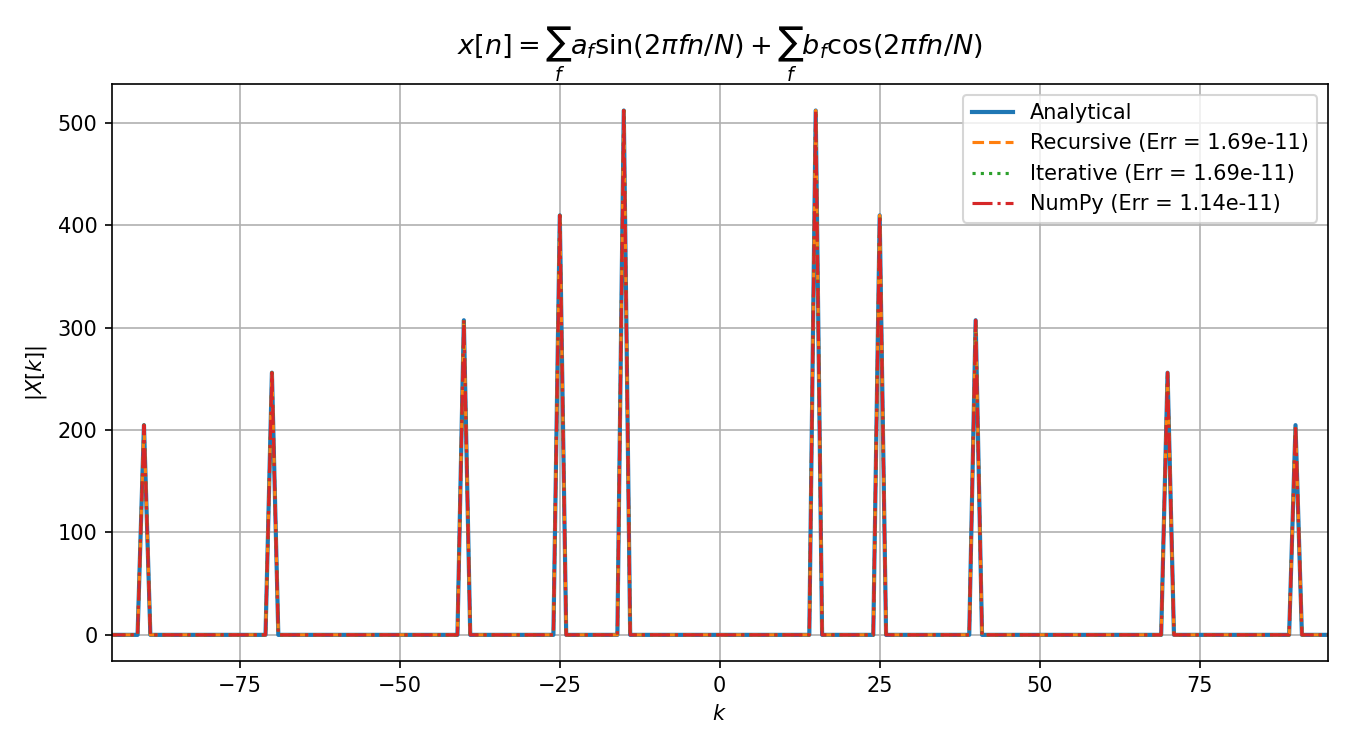
\includegraphics[width=1\linewidth]{../figures/sine_cosine.png}
    \caption{Comparación de la DFT implementada con los códigos descritos en la sección \ref{intro}, la dada por la rutina \texttt{np.fft()} y la solución analítica de una función combinación de senos y cosenos. Se han tomado $N = 1024$ puntos para discretizar la función. El error se mide como la norma $L^2$.}
    \label{senoycoseno}
\end{figure}



\subsection{Gaussianas}

\begin{figure}[H]
    \centering
    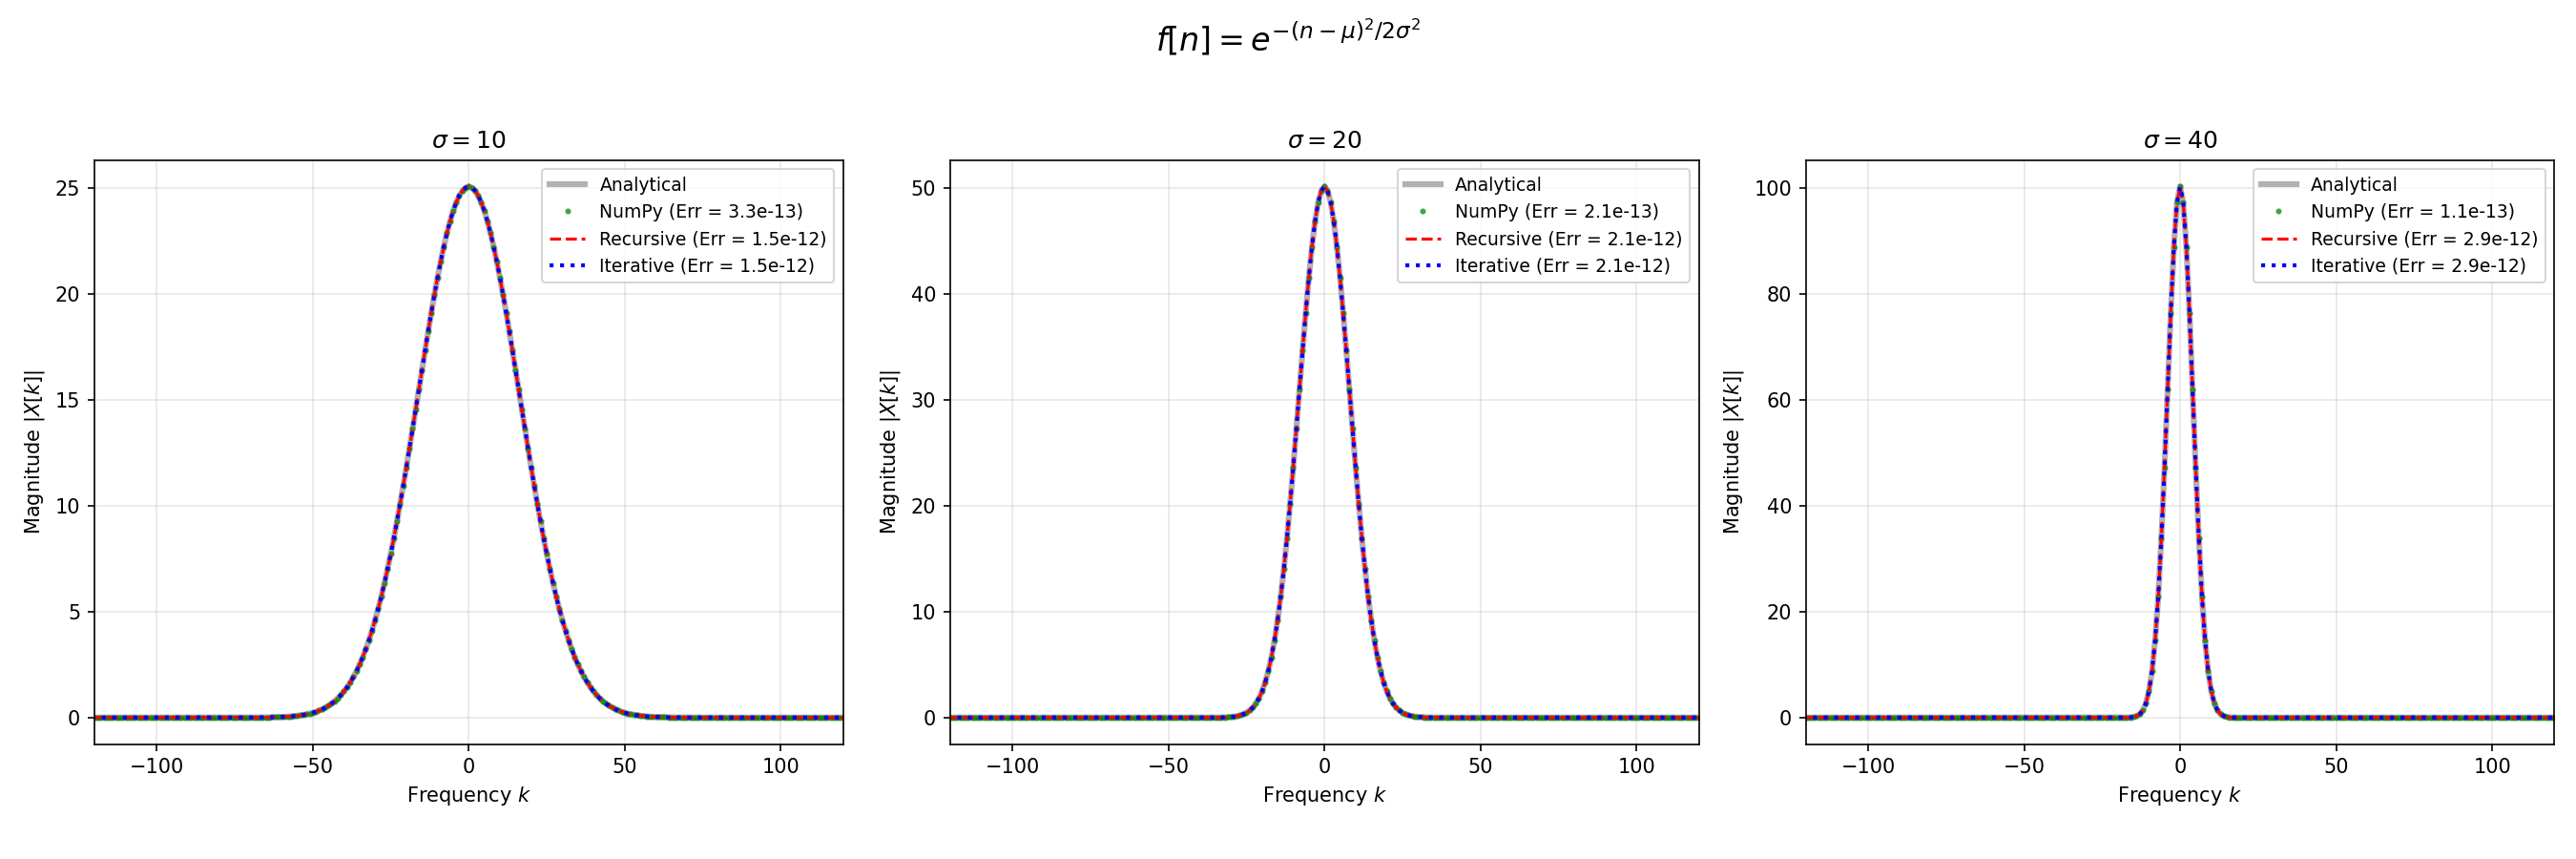
\includegraphics[width=1\linewidth]{../figures/gaussians.png}
    \caption{Comparación de la DFT implementada con los códigos descritos en la sección \ref{intro}, la dada por la rutina \texttt{np.fft()} y la solución analítica de funciones gaussianas. Se han tomado $N = 1024$ puntos para discretizar la función. El error se mide como la norma $L^2$.}
    \label{gaussianas}
\end{figure}



\subsection{Deltas de Kronecker}

\begin{figure}[H]
\centering

\begin{subfigure}{0.8\textwidth}
    \centering
    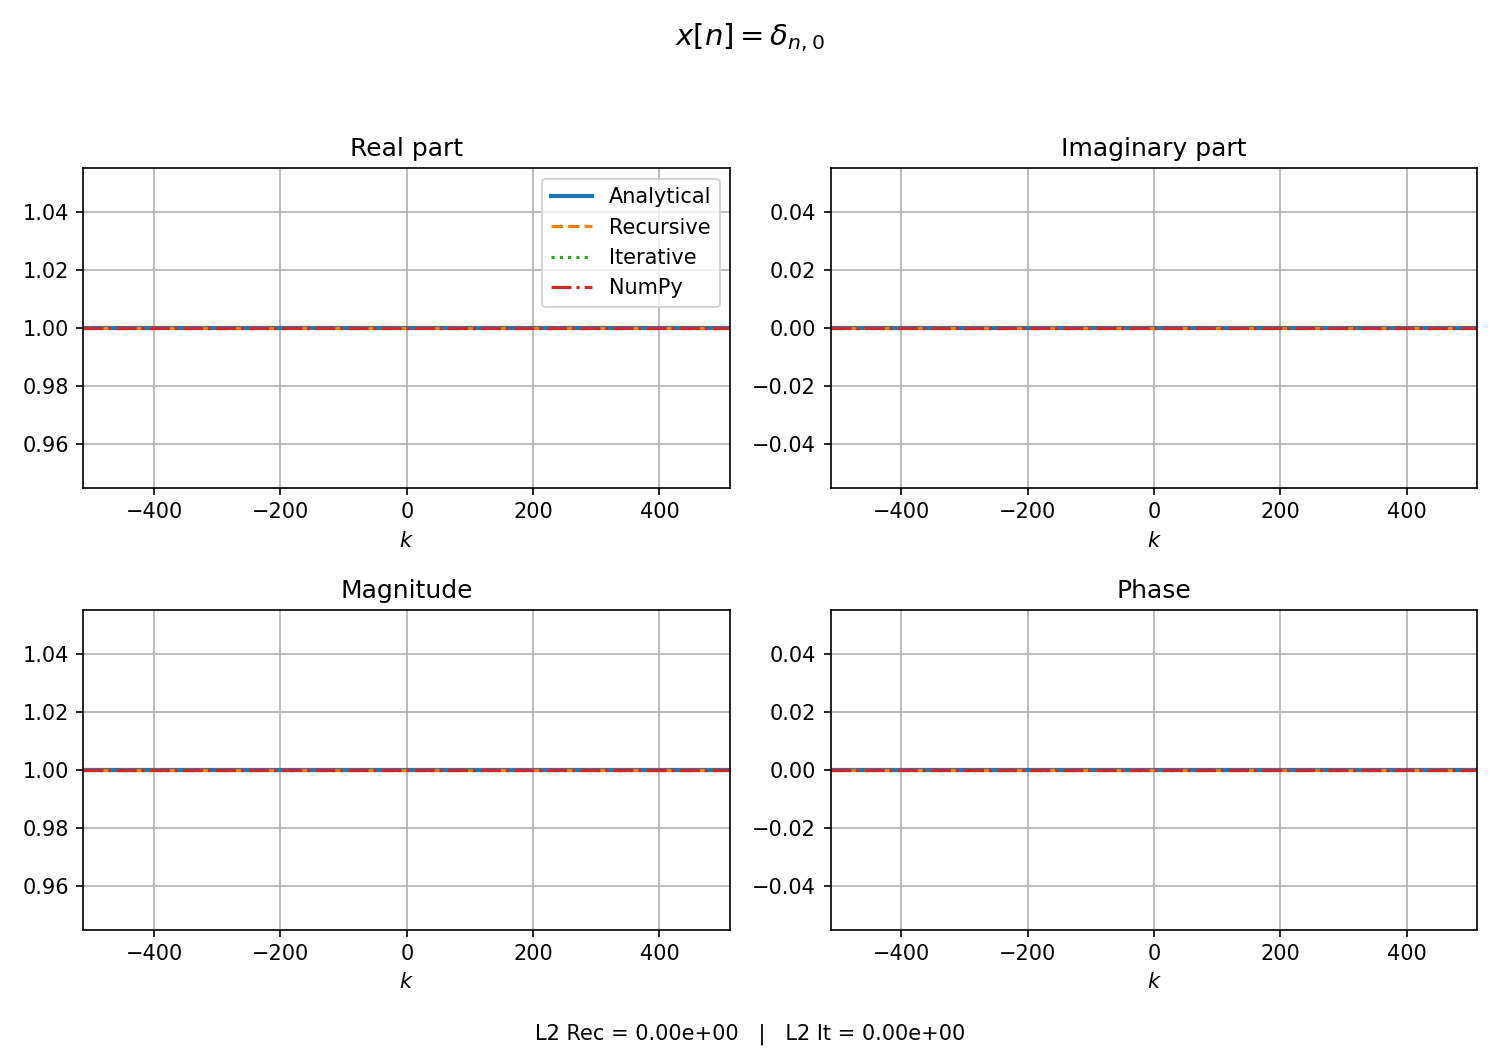
\includegraphics[width=\linewidth]{../figures/delta0.png}
    \caption{$\delta_{n,0}$}
\end{subfigure}

\vfill

\begin{subfigure}{0.8\textwidth}
    \centering
    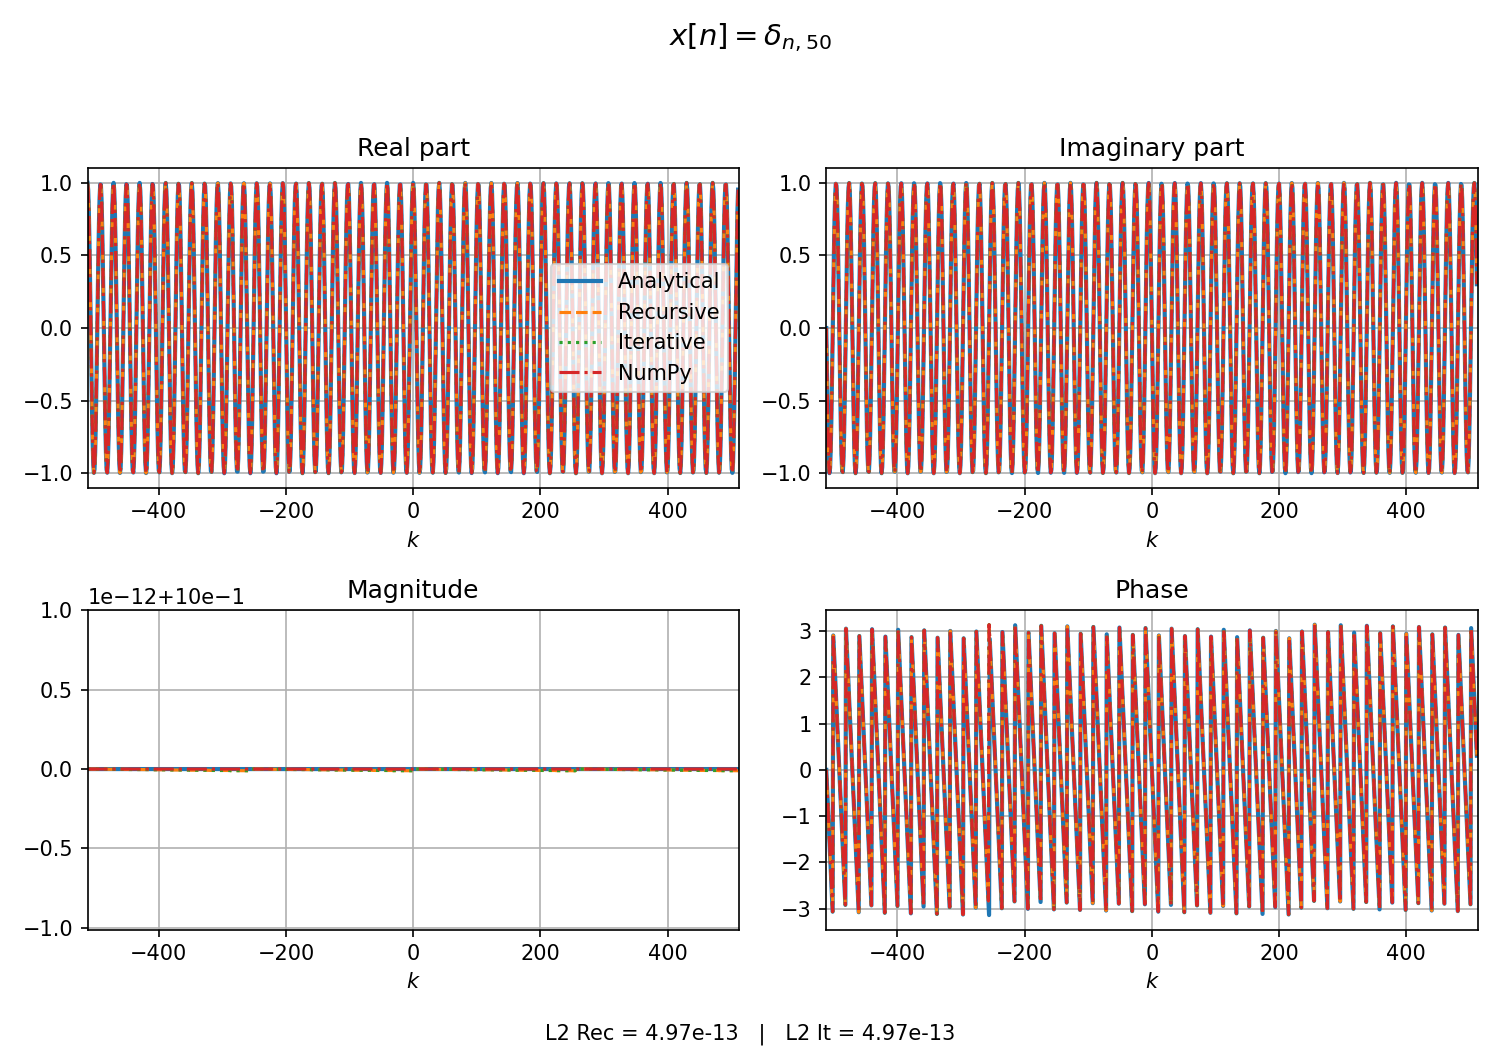
\includegraphics[width=\linewidth]{../figures/delta50.png}
    \caption{$\delta_{n,50}$}
\end{subfigure}

\caption{Comparación de la DFT implementada con los códigos descritos en la sección \ref{intro}, la dada por la rutina \texttt{np.fft()} y la solución analítica de funciones delta de Kronecker. Se han tomado $N = 1024$ puntos para discretizar la función. El error se mide como la norma $L^2$.}
\end{figure}



\subsection{Pulso cuadrado}

\begin{figure}[H]
    \centering
    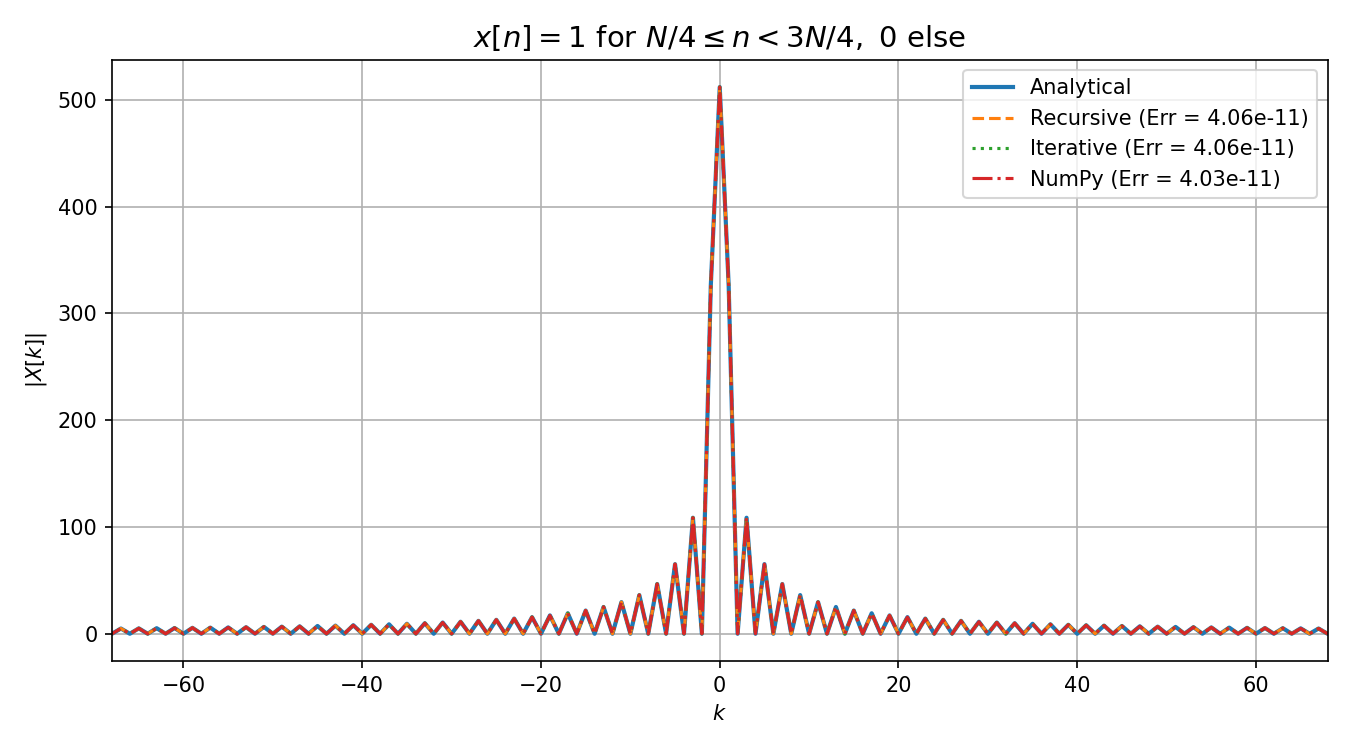
\includegraphics[width=1\linewidth]{../figures/square_pulse.png}
    \caption{Comparación de la DFT implementada con los códigos descritos en la sección \ref{intro}, la dada por la rutina \texttt{np.fft()} y la solución analítica de un pulso cuadrado. Se han tomado $N = 1024$ puntos para discretizar la función. El error se mide como la norma $L^2$.}
\end{figure}



\subsection{Función constante}

\begin{figure}[H]
    \centering
    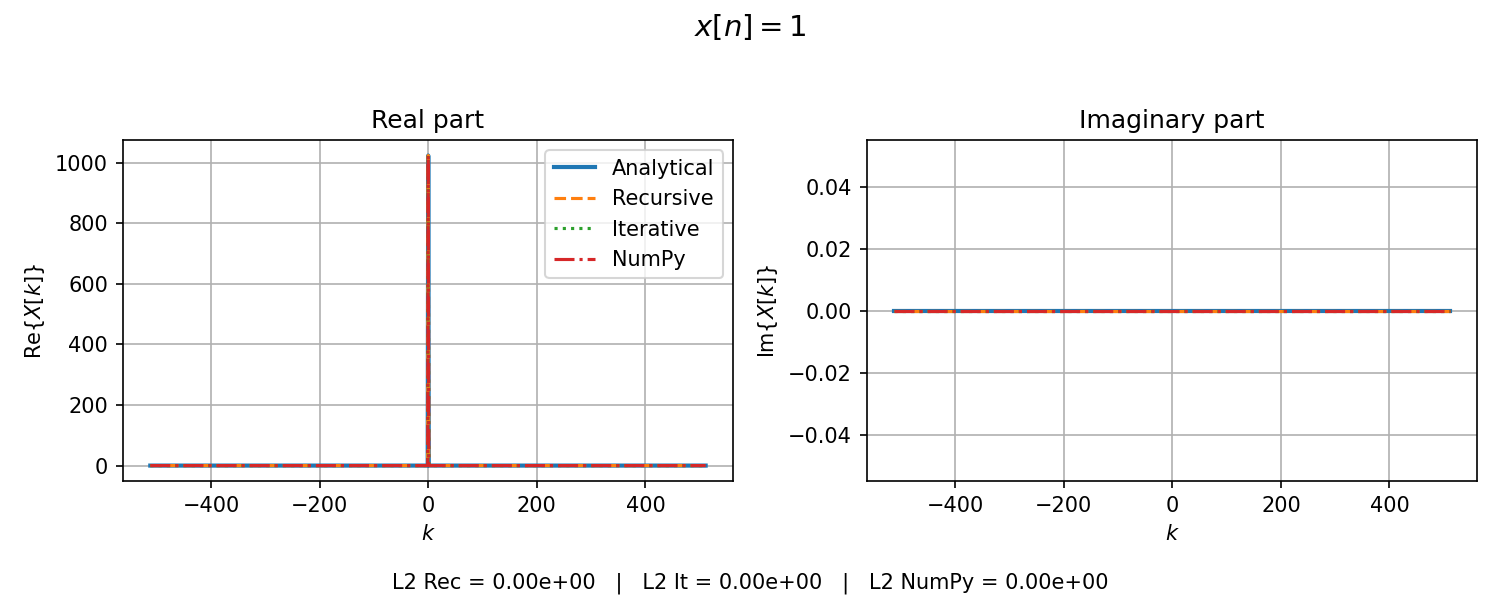
\includegraphics[width=1\linewidth]{../figures/constant.png}
    \caption{Comparación de la DFT implementada con los códigos descritos en la sección \ref{intro}, la dada por la rutina \texttt{np.fft()} y la solución analítica de una constante. Se han tomado $N = 1024$ puntos para discretizar la función. El error se mide como la norma $L^2$.}
\end{figure}



\subsection{Onda plana}

\begin{figure}[H]
    \centering
    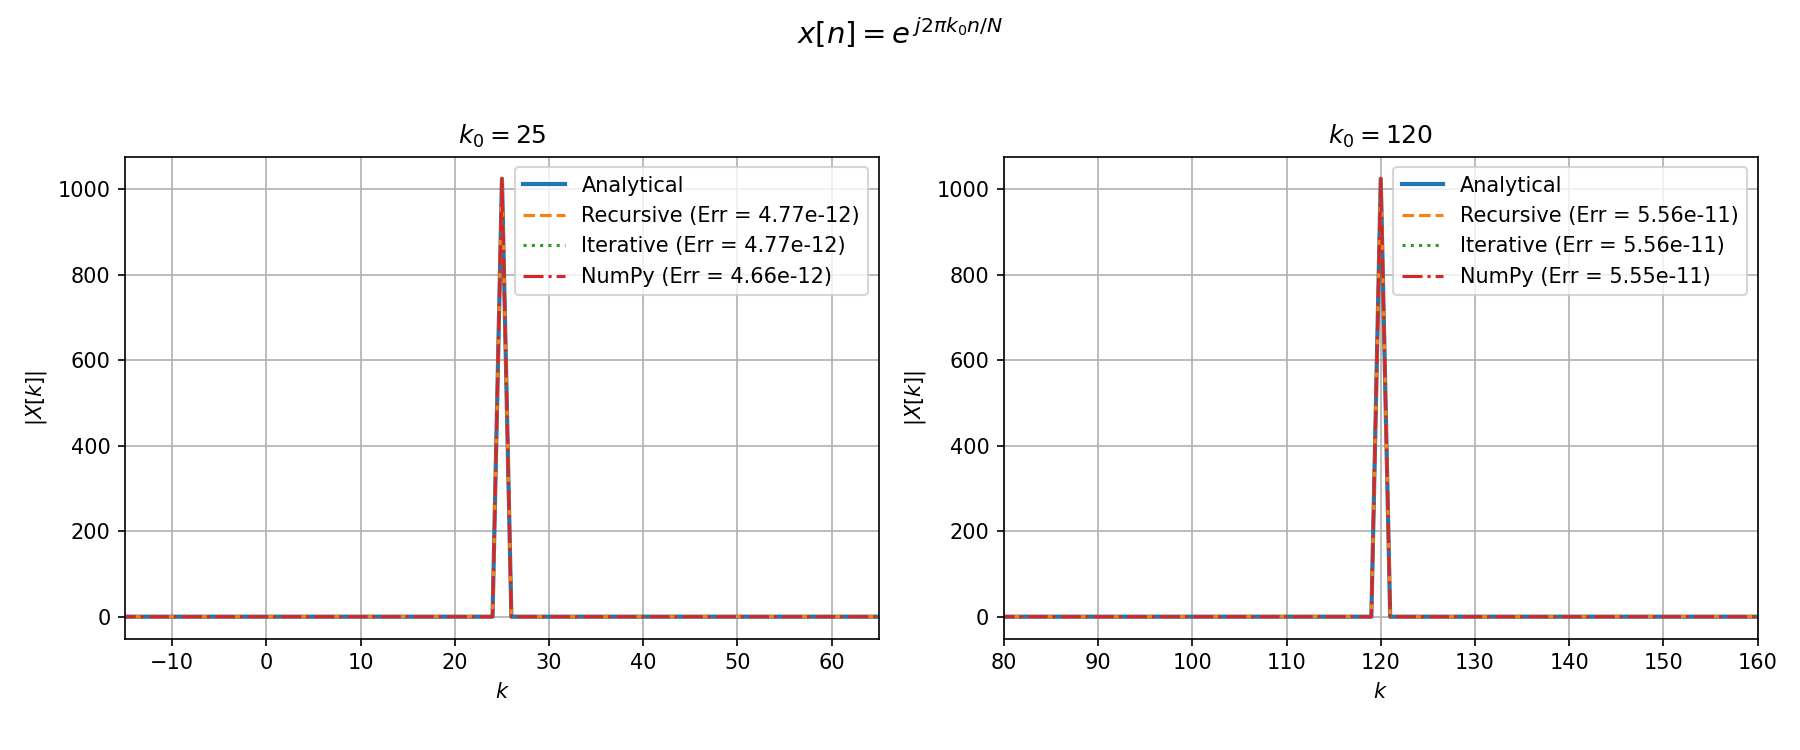
\includegraphics[width=1\linewidth]{../figures/plane_wave.png}
    \caption{Comparación de la DFT implementada con los códigos descritos en la sección \ref{intro}, la dada por la rutina \texttt{np.fft()} y la solución analítica de una onda plana compleja $x[n]=e^{j2\pi k_0 n/N}$. Se han tomado $N = 1024$ puntos para discretizar la función. El error se mide como la norma $L^2$.}
\end{figure}




\section{Verificación de propiedades de la FFT}


La transformada de Fourier teórica verifica las siguientes propiedades

\begin{itemize}
    \item $\mathcal{F}\mathcal{F}^{-1} =\mathcal{F}^{-1}\mathcal{F} = \mathcal{I}$,
    \item $\mathcal{F}^4 = N^2 \, \mathcal{I}$,
    \item Conservación de la norma (Parseval).
\end{itemize}


En la siguiente gráfica se muestra el error medido en norma $L^2$ de cada una de las propiedades descritas. Se observa que pese a aumentar con $N$ el error se mantiene del orden de $10^{-11}$, por lo que las propiedades teóricas se verifican.


\newpage
\begin{figure}[H]
    \centering
    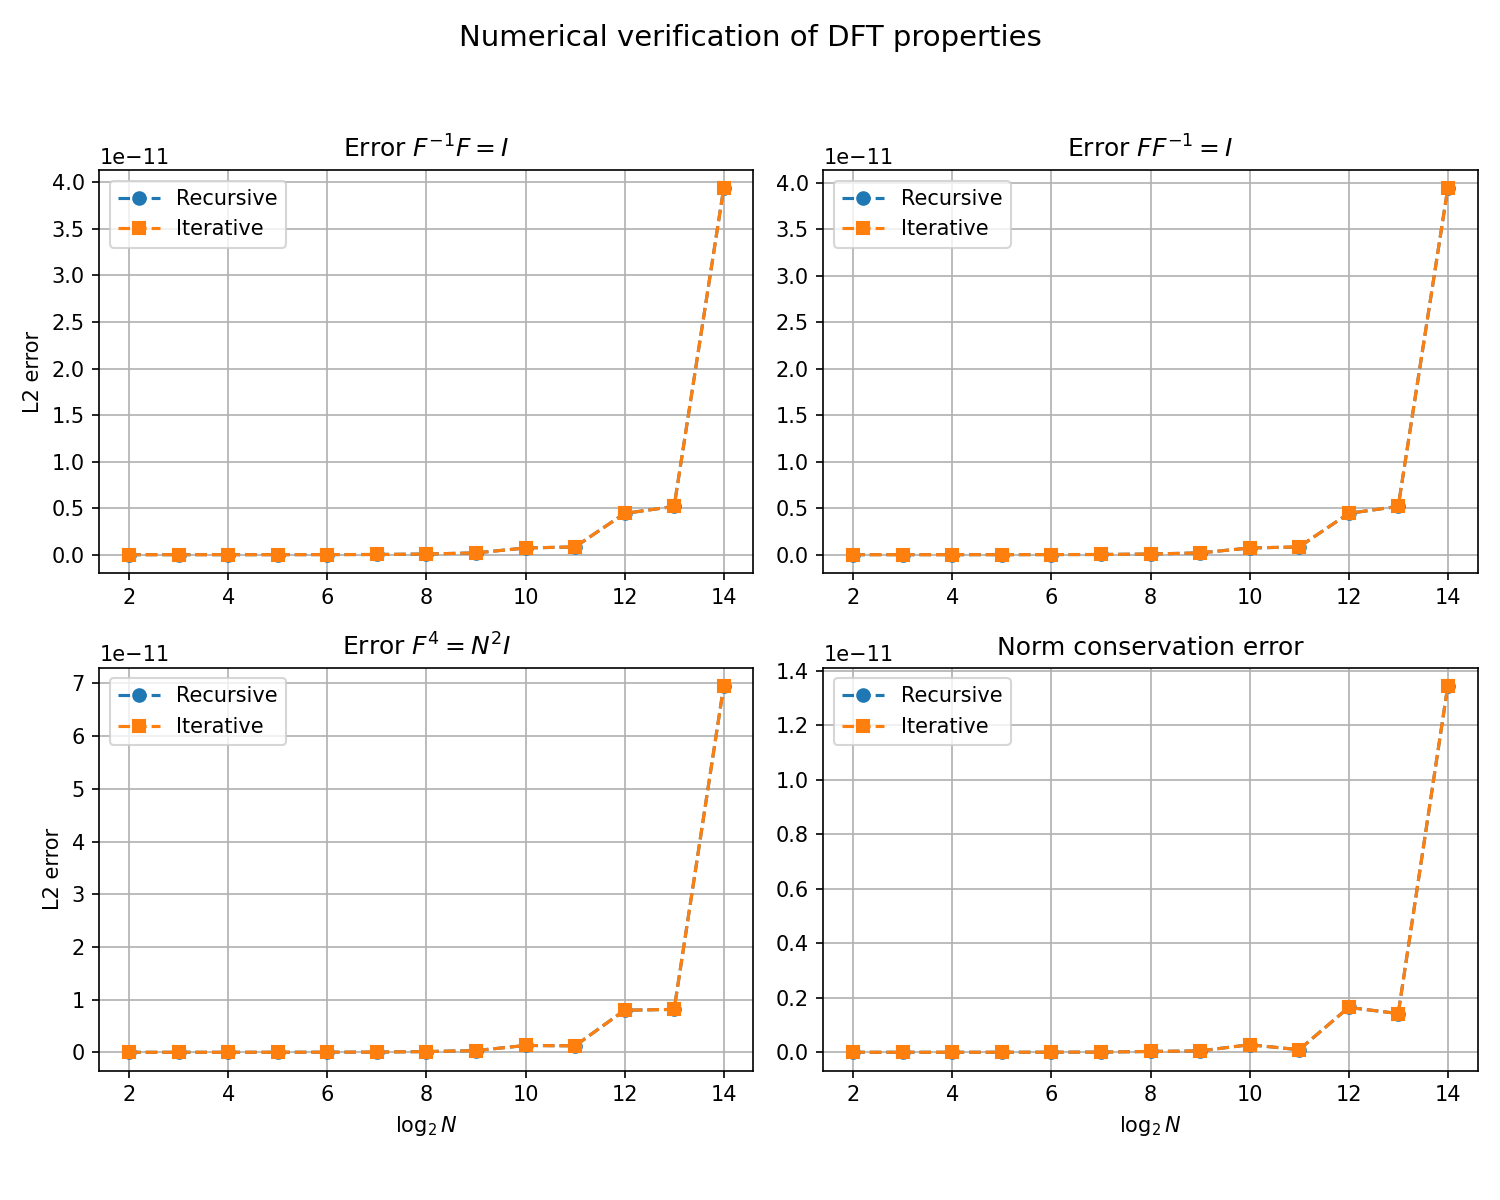
\includegraphics[width=0.8\linewidth]{../figures/properties.png}
    \caption{Comprobación de las propiedades teóricas de la DFT implementada con los códigos descritos en la sección \ref{intro}. Se ha tomado como señal un vector complejo aleatorio con componentes distribuidas según una normal de media 0 y varianza 1. Los resultados se promediaron sobre $10^2$ realizaciones. El eje $x$ está en escala $\log_2 N$. El error se mide como la norma $L^2$.}
\end{figure}


La última comprobación es el tiempo de ejecución, que tiene una complejidad de orden $\mathcal{O} (N\log_2N)$. Como se puede observar en la siguiente gráfica, al normalizar el tiempo por $N\log_2N$ se obtienen curvas constantes, lo que verifica que efectivamente el tiempo escala con $N\log_2N$. Además, no se aprecia una diferencia significativa en tiempo de ejecución entre el método recursivo e iterativo.



\begin{figure}[H]
    \centering
    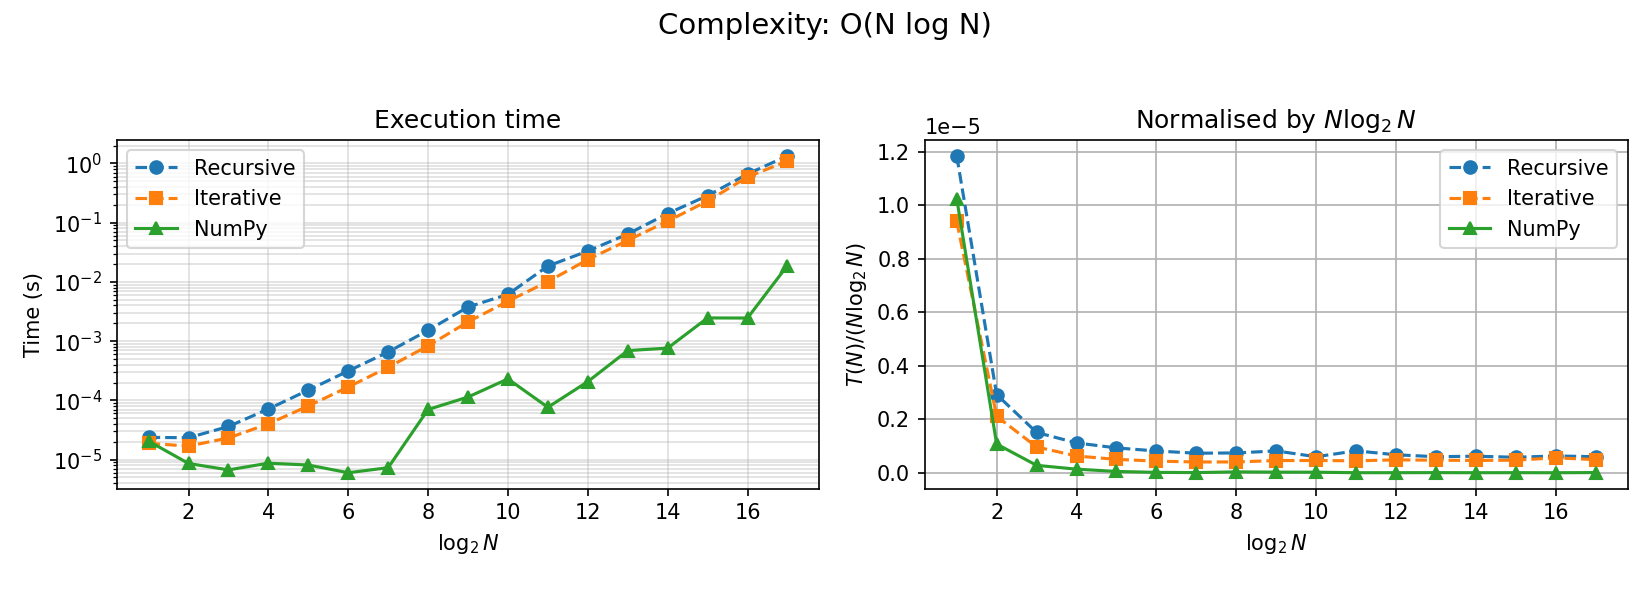
\includegraphics[width=1\linewidth]{../figures/timings.png}
    \caption{Comprobación del grado de complejidad la DFT implementada con los códigos descritos en la sección \ref{intro} y \texttt{np.fft()}. Se ha tomado como señal un vector complejo aleatorio con componentes distribuidas según una normal de media 0 y varianza 1.}
\end{figure}




\section{Transformada de Fourier en Física Cuántica}


La función de onda $\psi$ de un estado cuántico puede representarse tanto en el espacio de posiciones $x$ como en el espacio de momentos $p$. Ambas representaciones están relacionadas a través de la transformada de Fourier \cite{sakurai2020modern}

$$
    \phi(p) = \frac{1}{\sqrt{2\pi \hbar}} \int_{-\infty}^{+\infty} \psi(x) e^{-jpx/\hbar} dx,
$$

y su inversa

$$
    \psi(x) = \frac{1}{\sqrt{2\pi \hbar}} \int_{-\infty}^{+\infty} \phi(p) e^{jpx/\hbar} dp.
$$


\subsection{Caso estacionario}

La ecuación de Schrödinger estacionaria para una partícula en una dimensión viene dada por

\begin{equation}
\hat H \psi(x) = E \psi(x),
\end{equation}

donde el Hamiltoniano es

\begin{equation}
\hat H =
-\frac{\hbar^2}{2m}\frac{d^2}{dx^2}
+ V(x).
\end{equation}

El operador cinético contiene una derivada segunda, que resulta costosa de evaluar directamente en el espacio real al involucrar puntos $x_{n+1}$, $x_{n}$ y $x_{n-1}$. Sin embargo, en el espacio de Fourier es muy sencillo de evaluar

\begin{equation}
\frac{d^2}{dx^2} \longleftrightarrow -k^2,
\end{equation}

por lo que el operador cinético se vuelve diagonal en dicha representación. Se puede así llevar $\psi(x)$ al espacio de momentos mediante una transformada de Fourier, evaluar el operador cinético en dicho espacio (donde es diagonal) y volver al espacio real con una transformada inversa. Es decir

\begin{equation}
\hat T
=
\mathcal F^{-1}
\left(
\frac{\hbar^2 k^2}{2m}
\right)
\mathcal F.
\end{equation}


Por otro lado, el potencial actúa en el espacio de posiciones como

\begin{equation}
(\hat V\psi)(x)=V(x)\psi(x),
\end{equation}

es decir, ya es diagonal. El Hamiltoniano discreto completo queda entonces

\begin{equation}
H = F^{-1} D F + V.
\end{equation}


\subsection{Caso dependiente del tiempo}


En problemas de evolución la función de onda a tiempo $t$ tiene solución formal

$$
    \psi(t) = e^{-j\hat{H}t/\hbar} \psi_0.
$$


El problema es que los operadores $\hat{T}$ y $\hat{V}$ no suelen conmutar. En este caso se utiliza la aproximación de tiempo corto

$$
    \psi(t + \Delta t) = e^{-j\hat{H}\Delta t/\hbar} \psi(t),
$$


donde el operador de evolución temporal se evalúa usando la aproximación de Trotter \cite{kalos2008monte}

$$
    e^{-j\hat{H}\Delta t/\hbar} = e^{-j\hat{T}\Delta t/2\hbar} e^{-j\hat{V}\Delta t/\hbar} e^{-j\hat{T}\Delta t/ 2\hbar} + \mathcal{O} (\Delta t^3).
$$


De esta forma el esquema de resolución queda como

\begin{itemize}
    \item [1.] $\psi(x) \to \phi(p)$ con una FFT
    \item [2.] Multiplicar por fase cinética
    \item [3.] $\phi'(p) \to \psi'(x)$ con una IFFT
    \item [4.] Multiplicar por fase potencial
    \item [5.] $\psi''(x) \to \phi''(p)$ con una FFT
    \item [6.] Multiplicar por fase cinética
    \item [7.] $\phi'''(p) \to \psi'''(x)$ con una IFFT
\end{itemize}


\subsection{Ejemplo: estado fundamental del oscilador armónico}

Como aplicación concreta se calcula la energía del estado fundamental del oscilador armónico cuántico unidimensional. En unidades naturales ($\hbar = m = \omega = 1$) el Hamiltoniano es

$$
\hat H = -\tfrac{1}{2}\frac{d^2}{dx^2} + \tfrac{1}{2} x^2,
$$

con autovalor fundamental exacto $E_0 = 1/2$ y autofunción $\psi_0(x) = \pi^{-1/4} e^{-x^2/2}$.

Se emplea el método \emph{split-operator} en tiempo imaginario: sustituyendo $t \to -i\tau$ en el operador de evolución, la exponencial $e^{-\hat H \tau}$ filtra las componentes de mayor energía, de modo que toda función de onda inicial con solapamiento no nulo con el estado fundamental converge a él. El operador cinético se aplica mediante FFT como se describió arriba.

\begin{figure}[H]
    \centering
    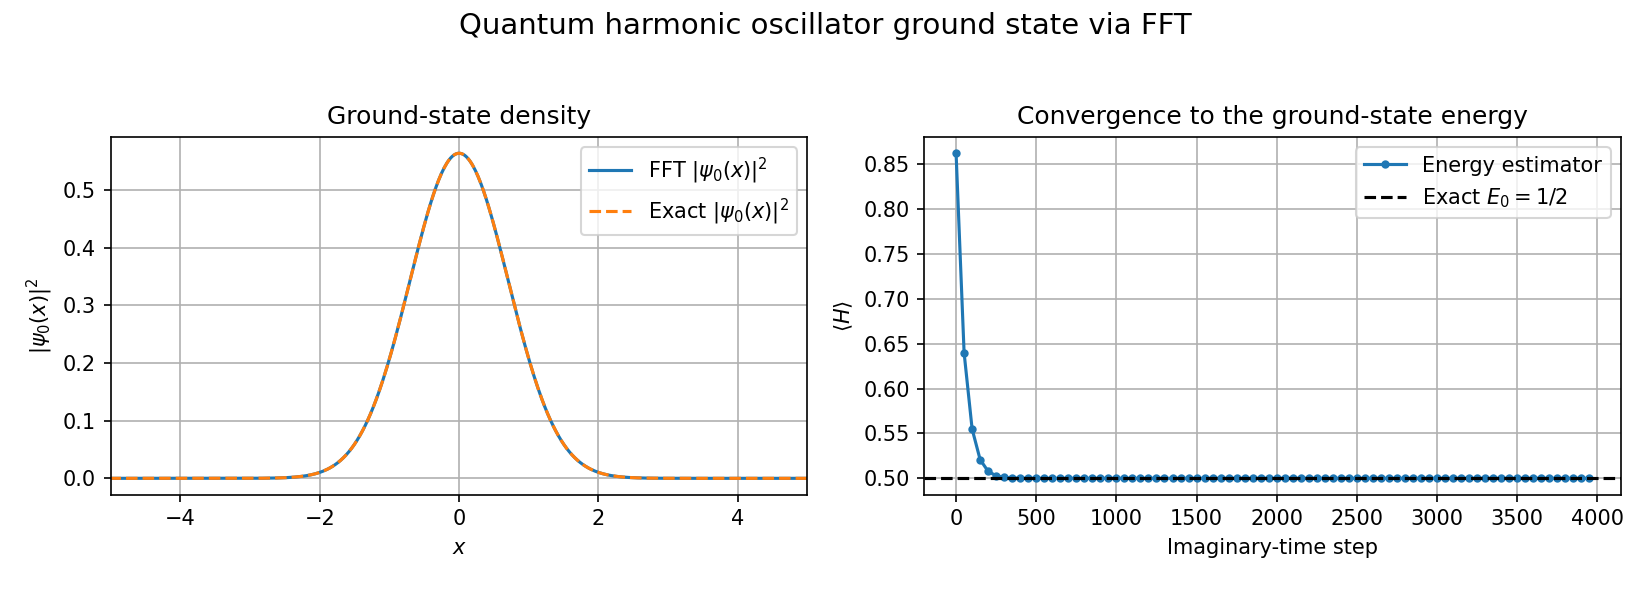
\includegraphics[width=1\linewidth]{../figures/harmonic_oscillator.png}
    \caption{Estado fundamental del oscilador armónico cuántico obtenido mediante propagación en tiempo imaginario con el método \emph{split-operator} basado en FFT. Izquierda: densidad de probabilidad $|\psi_0(x)|^2$ numérica frente a la gaussiana analítica $\pi^{-1/2} e^{-x^2}$. Derecha: convergencia del estimador de energía $\langle H \rangle$ al valor exacto $E_0 = 1/2$.}
\end{figure}



\newpage
\section{Conclusión}



Se ha estudiado la transformada discreta de Fourier y su implementación eficiente mediante el algoritmo de transformada rápida de Fourier (FFT) que permite reducir el coste original $\mathcal{O}(N^2)$ a un orden $\mathcal{O}(N\log_2 N)$ mediante una descomposición recursiva basada en la separación de índices pares e impares.

Desarrollando dos implementaciones propias del algoritmo FFT, una versión recursiva y otra iterativa basada en el procedimiento de \emph{bit-reversal}, se observa que ambas coinciden con la rutina \texttt{np.fft()} de la librería NumPy y con las soluciones analíticas para diversas funciones representativas. En todos los casos, los resultados obtenidos presentan una excelente concordancia, con errores del orden de $10^{-10}$.

Asimismo, se ha comprobado numéricamente que los algoritmos implementados verifican las propiedades fundamentales de la transformada de Fourier, como la inversión, la conservación de la norma y la periodicidad de orden cuatro.

El estudio del tiempo de ejecución muestra que ambas versiones del algoritmo presentan un comportamiento compatible con la complejidad teórica $\mathcal{O}(N\log_2 N)$. Aunque la versión iterativa presenta ventajas en términos de uso de memoria, no se observan diferencias significativas en tiempo de ejecución para los tamaños considerados.

Finalmente, se ha explorado la aplicación de la transformada de Fourier en el contexto de la mecánica cuántica, analizando la relación entre las representaciones en posición y momento, así como la resolución numérica de la ecuación de Schrödinger mediante métodos espectrales. El uso de la FFT permite evaluar de forma eficiente el operador cinético y construir el Hamiltoniano discreto, obteniendo niveles de energía y autofunciones con alta precisión, como se ha mostrado para el oscilador armónico cuántico.



\newpage
\bibliographystyle{plain}
\bibliography{bibliography}




\end{document}
